\documentclass{article}
\usepackage[utf8]{inputenc}
\usepackage{graphicx}
\usepackage{apuntes-ucppm}
\usepackage{fancyhdr}
\usepackage{amsmath}
\usepackage{bookmark}
\usepackage[a4paper, margin=1.25in]{geometry}
\usepackage{tikz}
\usepackage{calc}

\usetikzlibrary{positioning,matrix, patterns,decorations.pathreplacing}

\title{Vectores C++ STL}
\logo{logo.png}
\author{Jorge Hernández Palop}

\tikzset{
  pics/array/.style 2 args={
    code = {
        \foreach \x [count=\xi, evaluate=\x as \sep using #2*\xi] in #1 {
            \node [draw, minimum size=#2 cm] at (\sep, 0) {\x};
        }
    }
  },
  pics/borderless array/.style 2 args={
    code = {
        \foreach \x [count=\xi, evaluate=\x as \sep using #2*\xi] in #1 {
            \node [minimum size=#2 cm] at (\sep, 0) {\x};
        }
    }
  }
}

\begin{document}
    \maketitle
    \section{Introducción}
    \subsection{¿Qué es un vector?}

    Un \textbf{vector} es una \textbf{estructura de datos} que nos permite guardar \textbf{elementos de un mismo
    tipo} de manera \textbf{secuencial}. Es decir es una lista de elementos del mismo tipo. 

    Existen otros mecanismos que nos permiten hacer lo mismo, como los arrays. Pero la principal ventaja
    de los vectores es que podemos \textbf{aumentar y disminuir el tamaño de nuestro vector a lo largo de 
    la ejecución del programa}, algo imposible con los arrays.

    Para poder usar los vectores deberemos de \textbf{importalos de la librería estándar de C++} 
    por medio del siguiente comando \texttt{\#include <vector>}.
    
    \begin{figure}[h]
        \centering
        \begin{tikzpicture}
            \def\mylist{3, 4, 2, -1, 4, 1, 2, 3}
            \def\size{0.8}
            \draw pic (A)  {array={\mylist}{\size}};
            \draw node (B) [left = -1em of A]  {$v=$};
        \end{tikzpicture}
        \caption{Representación gráfica de un vector \texttt{v} de tamaño 8  de tipo \texttt{int}}
    \end{figure}

    \subsection{¿Cómo acceder a los elementos de un vector?}


    Para acceder a cada elemento de un vector se debe usar un \textbf{indice} que corresponde con la \textbf{posición
    del elemento} dentro del vector. En la mayoría de lenguajes de programación el indice \textbf{comienza en 0}
    y C++ no es la excepción.
    
    Para acceder a los elementos indicaremos el nombre del vector y el indice entre paréntesis,
    por ejemplo, \texttt{miVector[0]}. De esta manera podemos leer, modificar y operar con los elementos
    del vector como si se tratasen de variables comunes y corrientes. 

    Por medio del método \texttt{front} podemos acceder al primer elemento del vector de la siguiente manera 
    \texttt{miVector.front()} y con \texttt{back} al último de elemento de la misma manera \texttt{miVector.back()}.

    \textbf{IMPORTANTE:} Solo podemos usar indices que se encuentren en el rango $[0, \text{tamaño vector})$.
    Si tratamos de acceder elementos fuera del tamaño del vector lo más posible es que el programa explote.

    \begin{figure}[h]
        \centering
        \begin{tikzpicture}
            \def\mylist{3, 4, 2, -1, 4, 1, 2, 3}
            \def\index{$v[0]$, $v[1]$, $v[2]$, $v[3]$, $v[4]$, $v[5]$, $v[6]$, $v[7]$}
            \def\size{0.8}

            
            \draw  pic (A) {array={\mylist}{\size}};
            \draw node (B) [left = -1em of A]  {$v=$};
            \draw pic (C) [below = 1em of A] {borderless array={\index}{\size}};
            \end{tikzpicture}
        \caption{Indices del vector $v$}
    \end{figure}

    \subsection{¿Cómo se crea un vector?}

    Existen varias maneras de crear o inicializar un vector. Estas son algunas, la primera es usando el constructor
    por defecto. De esta manera creamos un vector de tamaño 0 con el tipo (\texttt{int, string, long long...}) que especifiquemos.
    $$\texttt{vector<tipoElementos> miVector;}$$

    La segunda manera es especificando el tamaño del vector antes de crearlo, de esta manera nos aseguraremos que el vector
    tenga un tamaño minimo antes de operar con él. Todos los elementos del vector pasarán a tener un valor por defecto
    que dependerá del tipo del vector, en el caso de los tipos númericos este valor será 0.

    $$\texttt{vector<tipoElementos> miVector(tamanoVector);}$$

    La tercera forma de crearlo es indicando un valor por defecto al vector además del tamaño. El resultado es el mismo
    que de la manera anterior, lo único que cambia es el valor por defecto con el que comienza cada elemento. 

    $$\texttt{vector<tipoElementos> miVector(tamanoVector, valorPorDefecto);}$$

    La última manera que se usa en programación competitiva es mediante inicialización de listas. Le pasamos una serie
    de elementos entre llaves al vector. El vector resultante tendra exactamente el tamaño de la lista que le hemos
    introducido y los elementos en el orden en el que se encontraban en la lista.

    $$\texttt{vector<tipoElementos> miVector \{elemento0, elemento1, ..., elementoN-1\};}$$

    \subsubsection{Ejemplos}

    \begin{figure}[h]
        \centering
        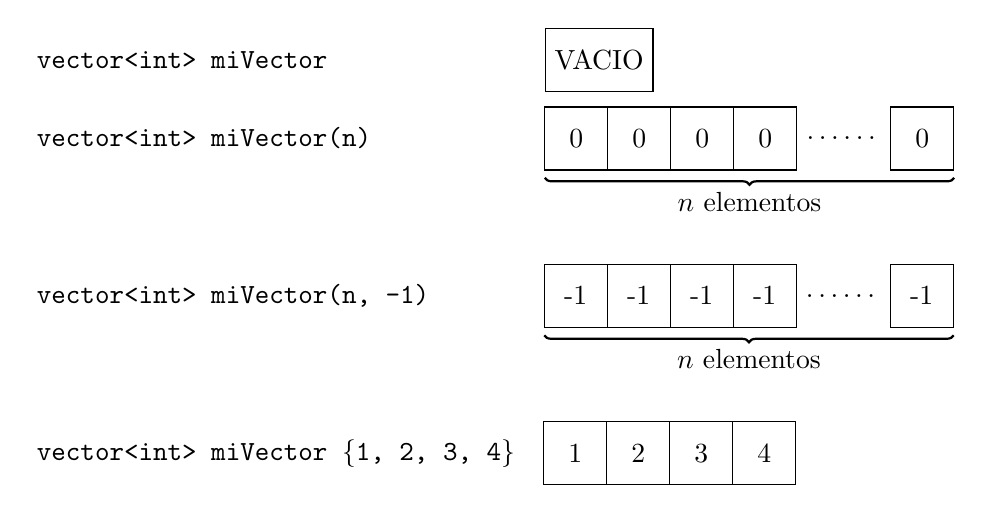
\begin{tikzpicture}
            % Defecto
            \draw node (vector1N) {\texttt{vector<int> miVector}};
            \draw node[draw, minimum size = 0.8cm, local bounding box=vector1, right = 7.5em of vector1N] {VACIO};
            
            \draw node[below = of vector1N.west, anchor=west] (vector2N) {\texttt{vector<int> miVector(n)}};
            \draw pic[below = of vector1.west, anchor=east, local bounding box=vector2] {array={{0, 0 , 0, 0}}{0.8}};
            \draw node[right = 0 of vector2] (vector2D) {\dots\dots};
            \draw node[draw, right = 0em of vector2D, minimum size = 0.8cm] (vector2M) {0};
            \draw [
            thick,
            decoration={
                brace,
                mirror,
                raise=0.5cm
            },
            decorate 
            ] (vector2.west) -- (vector2M.east) node [pos=0.5,anchor=north,yshift=-0.55cm] {$n$ elementos}; 

            \draw node[below = 2 of vector2N.west, anchor=west] (vector3N) {\texttt{vector<int> miVector(n, -1)}};
            \draw pic[below = 2 of vector2.west, anchor=east, local bounding box=vector3] {array={{-1, -1 , -1, -1}}{0.8}};
            \draw node[right = 0 of vector3] (vector3D) {\dots\dots};
            \draw node[draw, right = 0em of vector3D, minimum size = 0.8cm] (vector3M) {-1};
            \draw [
            thick,
            decoration={
                brace,
                mirror,
                raise=0.5cm
            },
            decorate 
            ] (vector3.west) -- (vector3M.east) node [pos=0.5,anchor=north,yshift=-0.55cm] {$n$ elementos}; 

            \draw node[below = 2 of vector3N.west, anchor=west] (vector4N) {\texttt{vector<int> miVector \{1, 2, 3, 4\}}};
            \draw pic[below = 2 of vector3.west, anchor=east, local bounding box=vector4] {array={{1, 2, 3, 4}}{0.8}};

        \end{tikzpicture}
        \caption{Distintos tipos de inicialización de vectores}
    \end{figure}

    \subsection{Notas Extras}

    \textit{En muchos problemas nos darán el tamaño del vector antes de decirnos sus elementos, en estos casos crear un 
    vector vacio de tamaño n es nuestra mejor opción ya aunque como veremos más adelante aumentar el tamaño del vector mientras
    insertamos elementos en un vector es 'rápido', esto supone un coste extra y hará que nuestro programa corra más rápido. 
    Por lo tanto el 75\% de las veces  va a ser mejor inicializar un vector con un tamaño n, antes que ir insertando elementos poco a poco. }
    \pagebreak
    \section{Operaciones}

    Ya hemos visto algunas operaciones básicas de los vectores, cómo crearlos y cómo acceder a sus elementos. Ahora veremos
    otras operaciones igual de importantes.

    \subsection{Obtener el tamaño de un vector}

    Para obtener el tamaño de un vector usamos el \texttt{size} que nos un numero entero sin signo. 
    También existe el método \texttt{empty} que devuelve \texttt{true} si y solo si el vector está 
    vacio, es decir, no tiene elementos.

    \begin{codelisting}{Tamaño de un vector}
    vector<int> v {3, 4, -1, 2};

    cout << v.size() << endl; // 4
    cout << v.empty() << endl; // false

    \end{codelisting}


    \textbf{IMPORTANTE:} \texttt{size} devuelve un número entero sin signo asi que hay que tener cuidado con las
    restas. Por ejemplo:

    \begin{codelisting}{Cuidado con los unsigned en \texttt{size()}}
vector<int> v;

// Este bucle falla 0 - 1 unsigned = 2^63 - 1
for(int i = 0; i < v.size() - 1; i++) {
    cout << i << " ";
}
cout << v[v.size() - 1] << endl;

// Este bucle no falla 0 - 1 signed = -1
for(int i = 0; i < (int) v.size() - 1; i++) {
    cout << i << " ";
}
cout << v[v.size() - 1] << endl;

\end{codelisting}


    \subsection{Leer vectores de la entrada estándar}

    Hemos visto que podemos inicializar el vector con valores por defecto o por medio de una lista. Sin embargo queremos
    poder cambiar esos valores según la entrada del problema para ello veremos dos maneras.

    La primera manera es asegurándonos de que tenemos el espacio suficiente para todos los elementos dentro del vector
    y por medio de un bucle ir leyendo de la entrada e ir rellenando el vector.

    \begin{codelisting}{Leer un vector de la entrada estándar 1}
int numeroElementos;
cin >> numeroElementos;

vector<int> v(numeroElementos);
for(int i = 0; i < numeroElementos; i++) {
    // Forma 1
    int x; 
    cin >> x; 
    v[i] = x;

    // Forma 2
    cin >> v[i];
}
    \end{codelisting}

    Otra formas menos recomendable, es inicializar un vector vacio e ir insertando elementos detrás por medio del método
    \texttt{push\_back}. Si hacemos \texttt{v.push\_back(elemento)} aumentaremos el tamaño del vector en uno e 
    insertaremos el nuevo elemento al final.

    \begin{codelisting}{Leer un vector de la entrada estándar 2}
    int numeroElementos;
    cin >> numeroElementos;
    
    vector<int> v;
    for(int i = 0; i < numeroElementos; i++) {
        int x; 
        cin >> x; 
        v.push_back(x);
    }
    \end{codelisting}

    \subsection{Insertar elementos}

    Existen dos opciones para insertar nuevos elementos dentro del vector. La primera opción es usar \texttt{push\_back},
    este método es muy rápido (tiene un coste amortizado de $\mathcal{O}(1)$). Se usa así \texttt{miVector.push\_back(elemento)} . Lo que hace es añadir el elemento al final 
    del vector. 
    
    El segundo método, es el método \texttt{insert} que nos permite seleccionar en que posición colocar el
    nuevo elemento, antes de ser colocado todos los elementos a la derecha se ruedan a una posición para poder hacer hueco
    al nuevo elemento. Este método es mucho más lento sobretodo cuando la posición sea cercana a 0 (tiene un coste de $\mathcal{O}(n)$). 
    Además hace uso de operadores, los cuales no hemos comentado. Se usa así \texttt{miVector.insert(iteradorEnLaPosicion, elemento)}. 
    Para determinar la posición del iterador vamos a usar \texttt{miVector.begin()}, que nos da un iterador al comienzo del vector, 
    y le sumamos la posición donde queremos insertar el elemento de la siguiente manera \texttt{miVector.insert(miVector.begin() + posición, elemento)}.
    
    Si no entiendes las operaciones con los iteradores no importa mucho ya que estas operaciones son muy poco frecuentes, sobretodo en vectores.
    \begin{figure}[h]
        \centering
        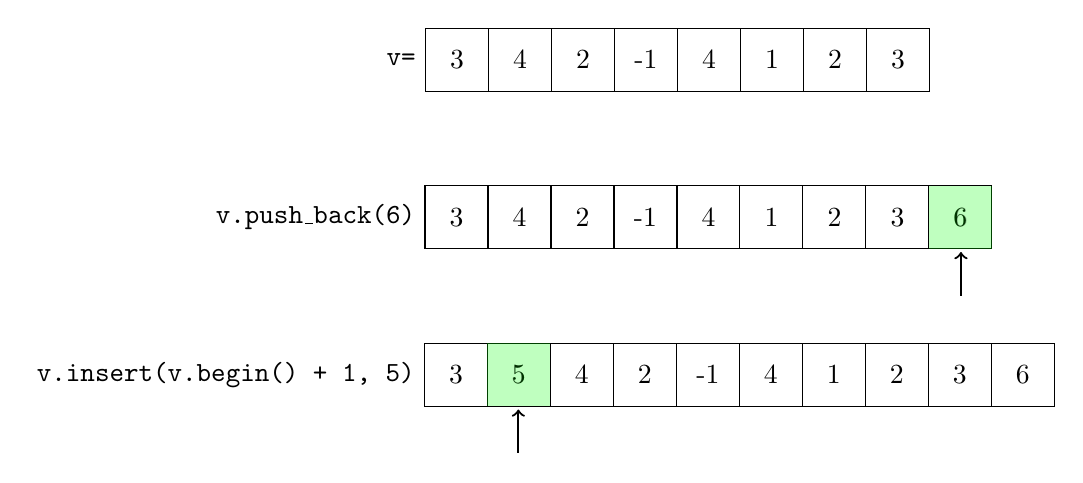
\begin{tikzpicture}
            \def\mylist{3, 4, 2, -1, 4, 1, 2, 3}
            \def\size{0.8}
            \draw pic [local bounding box=A] {array={\mylist}{\size}};
            \draw node (B) [left = 0em of A]  {\texttt{v=}};

            \def\mylist{3, 4, 2, -1, 4, 1, 2, 3, 6}
            \draw pic [below = 2 of A.west, anchor=east, local bounding box=C] {array={\mylist}{\size}};
            \draw node (D) [right = -0.8cm of C, minimum size = \size cm, fill=green, opacity=0.25] {6};
            \draw node (B) [left = 0em of C]  {\texttt{v.push\_back(6)}};
            \draw[thick,<-,shorten <=1pt] (D) -- +(-90:1cm);

            \def\mylist{3, 5, 4, 2, -1, 4, 1, 2, 3, 6}
            \draw pic [below = 2 of C.west, anchor=east, local bounding box=E] {array={\mylist}{\size}};
            \draw node (F) [left = -1.6cm of E, minimum size = \size cm, fill=green, opacity=0.25] {5};
            \draw node (G) [left = 0em of E]  {\texttt{v.insert(v.begin() + 1, 5)}};
            \draw[thick,<-,shorten <=1pt] (F) -- +(-90:1cm);
        \end{tikzpicture}
        \caption{Ejemplo de inserción de elementos con \texttt{push\_back} e \texttt{insert}}
    \end{figure}

    \begin{codelisting}{Inserción de elementos}
int n = 4;        
vector<int> v(n);
for(int i = 0; i < n; i++) {
    v[i] = i;
}
// v = {0, 1, 2, 3};

v.push_back(6); // v = {0, 1, 2, 3, 6};

auto it = v.begin() + 1;
v.insert(it, -1); // v = {0, -1, 1, 2, 3, 6};
        \end{codelisting}


    \subsection{Eliminar elementos}

    La eliminación de elementos aunque no es tan común en los problemas se puede hacer a través de dos métodos nuevamente
    \texttt{pop\_back} y \texttt{erase}. El método \texttt{pop\_back} permite la eliminación del último elemento del
    vector, es el opuesto del método \texttt{push\_back}. Este método es bastante rápido (tiene un coste amortizado de 
    $\mathcal{O}(1)$). Se usa así \texttt{miVector.pop\_back()}. El método \texttt{erase} es un método es más complejo 
    ya que hace uso de iteradores de la misma manera que lo hacía \texttt{insert}. Se usa así \texttt{miVector.erase(iteradorEnLaPosicion)},
    si tenemos la posición a eliminar podemos hacer lo siguiente \texttt{miVector.erase(miVector.begin() + posicionEliminar)}.
    Al igual que \texttt{insert} es más lento conforme la posición a borrar sea más cercana a 0, (tiene un coste de 
    $\mathcal{O}(n)$).

    \begin{figure}[h]
        \centering
        \begin{tikzpicture}
            \def\mylist{3, 4, 2, -1, 4, 1, 2, 3, 6}
            \def\size{0.8}
            \draw pic [local bounding box=A] {array={\mylist}{\size}};
            \draw node (B) [left = 0em of A]  {\texttt{v=}};

            \def\mylist{3, 4, 2, -1, 4, 1, 2, 3, 6}
            \draw pic [below = 2 of A.west, anchor=east, local bounding box=C] {array={\mylist}{\size}};
            \draw node (D) [right = -0.8cm of C, minimum size = \size cm, opacity=0.25] {6};
            \draw node (B) [left = 0em of C]  {\texttt{v.pop\_back()}};
            \draw [thick, red] (D.north west) -- (D.south east) (D.south west) -- (D.north east);
            \draw[thick,<-,shorten <=1pt] (D) -- +(-90:1cm);

            \def\mylist{3, 4, 2, -1, 4, 1, 2, 3}
            \draw pic [below = 2 of C.west, anchor=east, local bounding box=E] {array={\mylist}{\size}};
            \draw node (G) [left = 0em of E]  {\texttt{v.erase(v.begin() + 1)}};
            \draw [thick, red] (F.north west) -- (F.south east) (F.south west) -- (F.north east);
            \draw[thick,<-,shorten <=1pt] (F) -- +(-90:1cm);

        \end{tikzpicture}
        \caption{Ejemplo de inserción de elementos con \texttt{pop\_back} e \texttt{erase}}
    \end{figure}

    \begin{codelisting}{Eliminación de elementos}
int n = 6;        
vector<int> v(n);
for(int i = 0; i < 2 * n; i += 2) {
    v[i] = i;
}
// v = {0, 2, 4, 6, 8, 10};

v.pop_back(); // v = {0, 2, 4, 6, 8};

v.erase(v.begin() + 2); // v = {0, 2, 6, 8};
    \end{codelisting}

    \subsection{Vectores multidimensionales}

    Como dijimos antes los vectores pueden contener casi cualquier tipo de elemento. Entre este
    los tipos que pueden se encuentran ¡otros vectores! Podemos crear vectores que contengan vectores
    y así sucesivamente. Lo general en los problemas es que como mucho necesitemos insertar
    un vector de vectores de enteros por ejemplo, el tipo de este vector sería \texttt{vector<vector<int>>} 
    por ejemplo. Esto es común cuando estamos representado matrices o grafos (lo veremos a lo largo del grupo). 
    
    Como son vectores podemos hacer con ellos todas las operaciones que hemos mencionado antes ya sea en el vector
    externo como en cada uno de los vectores internos.

    Si queremos acceder a los elementos de los vectores internos usaremos dos veces el operador []. Con \texttt{miVector[y]}
    obtendremos el un vector de tipo \texttt{vector<tipoElemento>} y con un segundo [] de la siguiente manera 
    \texttt{miVector[y][x]} el elemento de tipo \texttt{tipoElemento} que se situa en la posición \texttt{x} del vector
    \texttt{y}.

    Cuando usamos vectores bidimensionales es preferible iterar sobre ellos primero recorriendo el vector interno antes
    de pasar a recorrer el siguiente vector. Si pensamos en una matriz (no es necesario que todas las filas tengan la misma longitud) a la que accedemos de la siguiente manera 
    \texttt{matriz[fila][columna]} es preferible recorrer todas las columnas antes de recorrer la siguiente fila

    \begin{figure}[h]
        \centering
        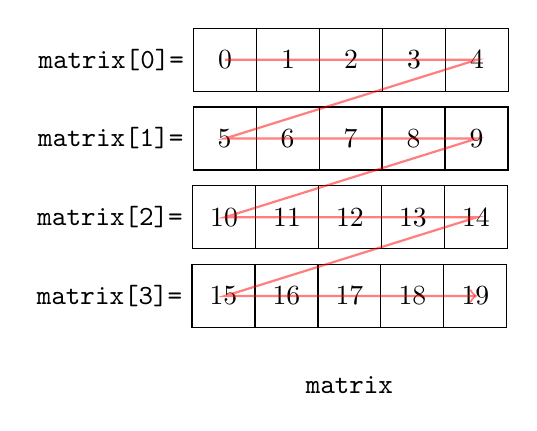
\begin{tikzpicture}
            \def\size{0.8}

            \def\mylist{0, 1, 2, 3, 4}
            \draw pic [local bounding box=A] {array={\mylist}{\size}};
            \draw node (AA) [left = 0em of A]  {\texttt{matrix[0]=}};

            \def\mylist{5, 6, 7, 8, 9}
            \draw pic [below = of A.west, anchor = east, local bounding box=B] {array={\mylist}{\size}};
            \draw node (BB) [left = 0em of B]  {\texttt{matrix[1]=}};

            \def\mylist{10, 11, 12, 13, 14}
            \draw pic [below = of B.west, anchor = east, local bounding box=C] {array={\mylist}{\size}};
            \draw node (CC) [left = 0em of C]  {\texttt{matrix[2]=}};

            \def\mylist{15, 16, 17, 18, 19}
            \draw pic [below = of C.west, anchor = east, local bounding box=D] {array={\mylist}{\size}};
            \draw node (DD) [left = 0em of D]  {\texttt{matrix[3]=}};

            \draw node (EE) [below = 0.5 of D]  {\texttt{matrix}};

            \draw [thick, red, opacity=0.5, ->] (0.8,0) -++ (0:3.2cm) -- (0.8,-1) -++ (0:3.2cm) -- (0.8,-2) -++ (0:3.2cm) -- (0.8,-3) -++ (0:3.2cm);

        \end{tikzpicture}
        \caption{Recorrido primero por columnas y luego por filas en un \texttt{vector<vector<int>>}}
    \end{figure}

    \begin{codelisting}{Ejemplo de Vectores multidimensionales}
// Creamos un vector de vectores vacios
vector<vector<int>> matriz;
int n = 4;
for(int fila = 0; fila < n; fila++) {
    matriz.push_back(vector<int>());
    for(int columna = 0; columna < n; columna++) {
        matriz[fila].push_back(columna + fila * n);
    }
}

// Segunda forma de crear una matriz
// Ya hemos declarado la variable antes
// si no seria vector<vector<int>> matriz(n, vector<int>(n));
matriz = vector<vector<int>>(n, vector<int>(n)); 
for(int fila = 0; fila < n; fila++) {
    for(int columna = 0; columna < n; columna++) {matrix[1]=
        matriz[fila][columna] = columna + fila * n;
    }
}

// Imprimos por pantalla la matriz
for(int fila = 0; fila < n; fila++) {
    for(int columna = 0; columna < n; columna++) {
        cout << matriz[fila][columna] << " ";
    }
    cout << endl;
}

/*
    0 1 2 3 
    4 5 6 7 
    8 9 10 11 
    12 13 14 15
*/
    \end{codelisting}

    \subsection{Ordenación de vectores}
    En muchos problemas es necesario ordenar el vector previamente como parte del algoritmo para resolverlo. 
    En FP se ven algoritmos de ordenación, sin embargo, son muy lentos (tienen complejidad $\mathcal{O}(n^2)$),
    la manera más rápida y relativamente eficiente (tiene coste $\mathcal{O}(n\log(n))$) de ordenar un vector en un concurso es por medio de la función
    \texttt{sort}. Le deberemos pasar el rango en el que queremos que ordene el vector por medio de iteradores de la 
    siguiente manera \texttt{sort(miVector.begin(), miVector.end())} y nos ordenará el vector de menor a mayor. Es importantes
    importar \texttt{algorithm} de la siguiente manera \texttt{\#include <algorithm>} para usar \texttt{sort}.

\begin{figure}[h]
        \centering
        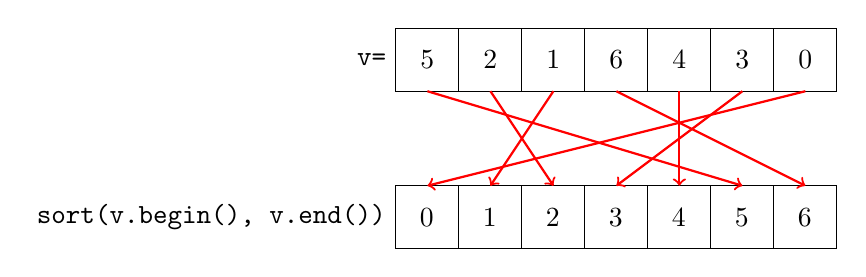
\begin{tikzpicture}
            \def\size{0.8}

            \def\mylist{5, 2, 1, 6, 4, 3, 0}
            \draw pic [local bounding box=A] {array={\mylist}{\size}};
            \draw node (AA) [left = 0em of A]  {\texttt{v=}};

            \def\mylist{0, 1, 2, 3, 4, 5, 6}
            \draw pic [below = 2 of A.west, anchor = east, local bounding box=B] {array={\mylist}{\size}};
            \draw node (BB) [left = 0em of B]  {\texttt{sort(v.begin(), v.end())}};

            \draw [thick, red, ->] (0.8,-0.4) -- (4.8, -1.6);
            \draw [thick, red, ->] (1.6,-0.4) -- (2.4, -1.6);
            \draw [thick, red, ->] (2.4,-0.4) -- (1.6, -1.6);
            \draw [thick, red, ->] (3.2,-0.4) -- (5.6, -1.6);
            \draw [thick, red, ->] (4.0,-0.4) -- (4.0, -1.6);
            \draw [thick, red, ->] (4.8,-0.4) -- (3.2, -1.6);
            \draw [thick, red, ->] (5.6,-0.4) -- (0.8, -1.6);


        \end{tikzpicture}
        \caption{Ordenación de un vector de enteros por medio de \texttt{sort}}
    \end{figure}

    Muchas veces nos interesa ordenar el vector de otra manera, por ejemplo de mayor a menor, para ello
    existe la función $\texttt{greater<tipoElemento>()}$ que usaremos de la siguiente manera 
    $\texttt{sort(miVector.begin(), miVector.end(), greater<tipoElemento>())}$. También podemos pasarle A
    sort nuestras propias funciones para ordenar siguiendo otros criterios
    siempre que sean de la forma $\texttt{bool miFuncion(tipoElemento a, tipoElemento b)}$. Donde $\texttt{miFuncion}$
    devuelve $ \texttt{true}$ si queremos que el elemento \texttt{a} se encuentre antes que \texttt{b}. Pasar
    una función de ordenación propia es especialmente útil cuando el vector no sea de enteros si no de pares o de
    algun tipo de dato que hemos creado nosotros, por ejemplo un intervalo, una esfera o lo que nos encontremos en los problemas.

    \begin{codelisting}{Ejemplo de ordenación}
// Los pares van primeros y luego ordenamos de mayor a menor
bool cmp(int a, int b) {
    return a % 2 == 0 && b % 2 == 1 || a > b;
}

int main() {
    vector<int> v {5, 2, 1, 6, 4, 3, 0};
    int n = 4;

    sort(v.begin(), v.end(), greater<int>());

    // 6 5 4 3 2 1 0
    for(int i = 0; i < v.size(); i++) cout << v[i] << " ";
    cout << endl;

    sort(v.begin(), v.end(), cmp);

    // 6 4 2 0 5 3 1
    for(int i = 0; i < v.size(); i++) cout << v[i] << " ";
    cout << endl;
}
    \end{codelisting}
    
    \subsection{Operaciones en vectores ordenados}
    En comun en muchos problemas el preguntar el menor o mayor elemento que cumple cierta condición para ayudarnos
    a resolver esos problemas en algunos casos podemos hacer uso de las funciones \texttt{lower\_bound} y 
    \texttt{upper\_bound}. Estas funciones operan sobre vectores ordenados y son muy rápidas (complejidad $\mathcal{O}(\log n)$). Necesitan
    de la librería \texttt{algorithm}.

    \texttt{lower\_bound} busca en la lista el \textbf{menor elemento que es mayor o igual a un elemento dado} y devuelve un iterador apuntando
    a la posición del elemento encontrado. Si ningún elemento cumple esa condición devuelve \texttt{miVector.end()}. Tambien podemos pasarle
    una función de comparación propia como en el caso del \texttt{sort}.

    \begin{figure}[h]
        \centering
        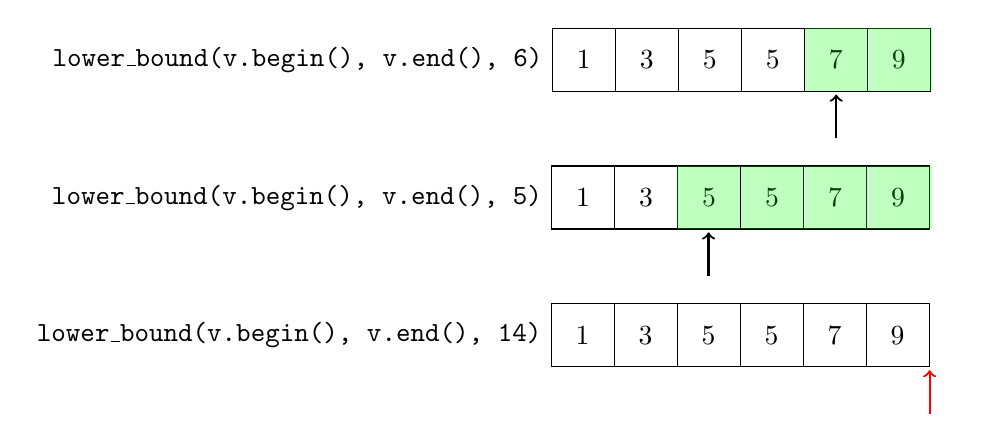
\begin{tikzpicture}
            \def\mylist{1, 3, 5, 5, 7, 9}
            \def\size{0.8}
            \draw pic [local bounding box=A] {array={\mylist}{\size}};
            \draw node (D) [right = -1.6cm of A, minimum size = \size cm, fill=green, opacity=0.25] {};
            \draw[thick,<-,shorten <=1pt] (D) -- +(-90:1cm);

            \draw node (B) [left = 0em of A]  {\texttt{lower\_bound(v.begin(), v.end(), 6)}};

            \draw node (DD) [right = 0 of D, minimum size = \size cm, fill=green, opacity=0.25] {};
            \draw pic [below = 1.75 of A.west, anchor=east, local bounding box=C] {array={\mylist}{\size}};
            \draw node (D) [left = -2.4cm of C, minimum size = \size cm, fill=green, opacity=0.25] {};
            \draw node (DD) [right = 0 of D, minimum size = \size cm, fill=green, opacity=0.25] {};
            \draw node (DDD) [right = 0 of DD, minimum size = \size cm, fill=green, opacity=0.25] {};
            \draw node (DDDD) [right = 0 of DDD, minimum size = \size cm, fill=green, opacity=0.25] {};
            \draw node (B) [left = 0em of C]  {\texttt{lower\_bound(v.begin(), v.end(), 5)}};
            \draw[thick,<-,shorten <=1pt] (D) -- +(-90:1cm);

            \draw pic [below = 1.75 of C.west, anchor=east, local bounding box=E] {array={\mylist}{\size}};
            \draw node (F) [right = -0.4cm of E, minimum size = \size cm, opacity=0.25] {};
            \draw node (G) [left = 0em of E]  {\texttt{lower\_bound(v.begin(), v.end(), 14)}};
            \draw[red, thick,<-,shorten <=1pt] (F) -- +(-90:1cm);
        \end{tikzpicture}
        \caption{Ejemplo de \texttt{lower\_bound}}
    \end{figure}

    \texttt{upper\_bound} busca en la lista el \textbf{menor elemento que es mayor a un elemento dado} y devuelve un iterador apuntando
    a la posición del elemento encontrado. Si ningún elemento cumple esa condición devuelve \texttt{miVector.end()}. Tambien podemos pasarle
    una función de comparación propia como en el caso del \texttt{sort}.

    \begin{figure}[h]
        \centering
        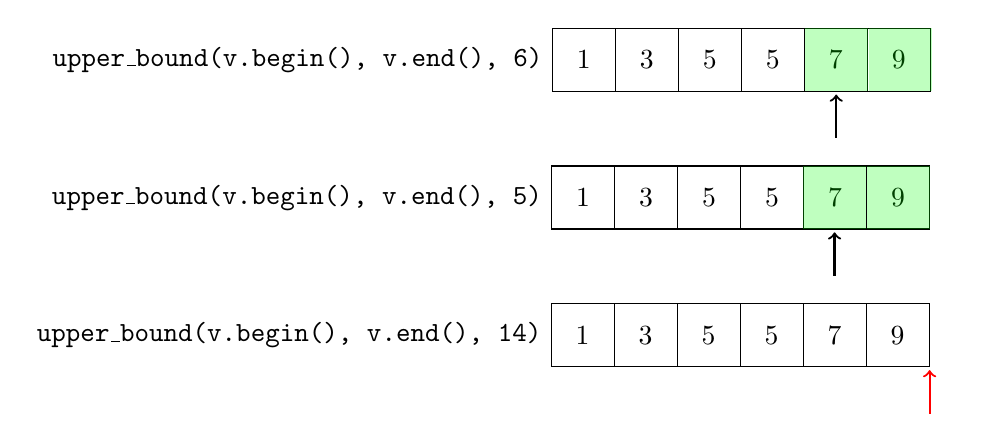
\begin{tikzpicture}
            \def\mylist{1, 3, 5, 5, 7, 9}
            \def\size{0.8}
            \draw pic [local bounding box=A] {array={\mylist}{\size}};
            \draw node (D) [right = -1.6cm of A, minimum size = \size cm, fill=green, opacity=0.25] {};
            \draw[thick,<-,shorten <=1pt] (D) -- +(-90:1cm);

            \draw node (B) [left = 0em of A]  {\texttt{upper\_bound(v.begin(), v.end(), 6)}};

            \draw node (DD) [right = 0 of D, minimum size = \size cm, fill=green, opacity=0.25] {};
            \draw pic [below = 1.75 of A.west, anchor=east, local bounding box=C] {array={\mylist}{\size}};
            \draw node (D) [left = -4cm of C, minimum size = \size cm, fill=green, opacity=0.25] {};
            \draw node (DD) [right = 0 of D, minimum size = \size cm, fill=green, opacity=0.25] {};
            \draw node (B) [left = 0em of C]  {\texttt{upper\_bound(v.begin(), v.end(), 5)}};
            \draw[thick,<-,shorten <=1pt] (D) -- +(-90:1cm);

            \draw pic [below = 1.75 of C.west, anchor=east, local bounding box=E] {array={\mylist}{\size}};
            \draw node (F) [right = -0.4cm of E, minimum size = \size cm, opacity=0.25] {};
            \draw node (G) [left = 0em of E]  {\texttt{upper\_bound(v.begin(), v.end(), 14)}};
            \draw[red, thick,<-,shorten <=1pt] (F) -- +(-90:1cm);
        \end{tikzpicture}
        \caption{Ejemplo de \texttt{upper\_bound}}
    \end{figure}
    \begin{codelisting}{Ejemplo de \texttt{lower\_bound} y \texttt{upper\_bound} }
vector<int> v {10, 10, 10, 20, 20, 20, 30, 30, 30};

auto lower = lower_bound (v.begin(), v.end(), 20);
auto upper = upper_bound (v.begin(), v.end(), 20);
int indiceLower = lower - v.begin();
int indiceUpper = upper - v.begin();

int elementoLower, elementoUpper;
if(lower != v.end())elementoLower = *lower;
else elementoLower = -1;    
if(upper != v.end())elementoUpper = *upper;
else elementoUpper = -1;    
cout << "lower: indice = " << indiceLower << ", elem = " << elementoLower << endl; 
cout << "upper: indice = " << indiceUpper << ", elem = " << elementoUpper << endl; 
/*10, 10, 10, 20, 20, 20, 30, 30, 30
               |           |
             lower       upper
    lower_bound: indice = 3, elemento = 20
    upper_bound: indice = 6, elemento = 30    */

lower = lower_bound (v.begin(), v.end(), 30);
upper = upper_bound (v.begin(), v.end(), 30);
indiceLower = lower - v.begin();
indiceUpper = upper - v.begin();

if(lower != v.end()) elementoLower = *lower;
else elementoLower = -1;    
if(upper != v.end()) elementoUpper = *upper;
else elementoUpper = -1;    
cout << "lower: indice = " << indiceLower << ", elem = " << elementoLower << endl; 
cout << "upper: indice = " << indiceUpper << ", elem = " << elementoUpper << endl; 
/*  10, 10, 10, 20, 20, 20, 30, 30, 30
                            |          |
                            lower      upper
    lower_bound: indice = 6, elemento = 30
    upper_bound: indice = 9, elemento = -1    */      
    \end{codelisting}
    \subsection{Invertir un vector}
    Este operación se encuentra dentro de la librería \texttt{algorithm} y nos permite invertir el orden de un vector
    de la siguiente manera \texttt{reverse(miVector.begin(), miVector.end())}.

    \begin{figure}[h]
        \centering
        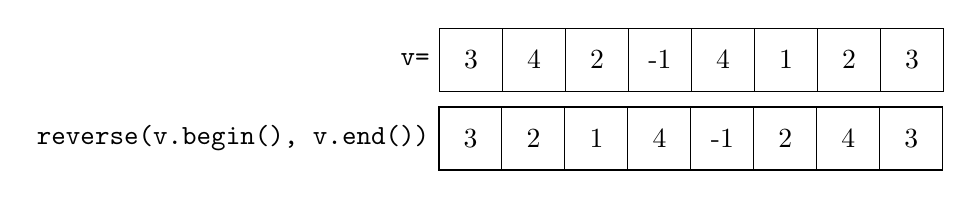
\begin{tikzpicture}
            \def\mylist{3, 4, 2, -1, 4, 1, 2, 3}
            \def\size{0.8}
            \draw pic [local bounding box=A] {array={\mylist}{\size}};
            \draw node (B) [left = 0em of A]  {\texttt{v=}};

            \def\mylist{3, 2, 1, 4, -1, 2, 4, 3}
            \def\size{0.8}
            \draw pic [below = of A.west, anchor = east, local bounding box=C] {array={\mylist}{\size}};
            \draw node (B) [left = 0em of C]  {\texttt{reverse(v.begin(), v.end())}};
        \end{tikzpicture}
        \caption{Ejemplo de operación \texttt{reverse}}
    \end{figure}

    \subsection{Iterar sobre un vector}
    Conocemos la manera típica de iterar sobre un vector por medio del bucle \texttt{for}.
    \begin{codelisting}{Iteración con \texttt{for} con indices}
vector<int> v {3, 4, 2, -1, 4, 1, 2, 3};
for(int i = 0; i < v.size(); i++) {
    cout << v[i] << " ";
} 
cout << endl; // 3 4 2 -1 4 1 2 3
    \end{codelisting}

    Sin embargo, existe una sintaxis que nos permite hacerlo escribiendo menos y es la siguiente
    \texttt{for(tipoElemento elemento : miVector) \{\}}. De esta manera obtenemos directamente el elemento
    en vez del indice del elemento.
    
    Esta notación nos permitirá iterar sobre otras estructuras donde
    no tenemos acceso directo a los elementos por medio de indices. 

    \begin{codelisting}{Iteración con \texttt{for} con iteradores}
vector<int> v {3, 4, 2, -1, 4, 1, 2, 3};
for(int i : v) {
    cout << i << " ";
} 
cout << endl; // 3 4 2 -1 4 1 2 3
    \end{codelisting}

    Finalmente en muchos problemas será necesario imprimir un vector como solución. El problema es que
    muchos jueces son muy rigurosos con la salida y no es posible insertar espacios al final de la salida
    como hemos hecho antes ya que nos dará Wrong Answer o Presentation Error. Por ello la forma más recomendable
    de imprimir un vector para dar una solución es:

    \begin{codelisting}{Imprimir un vector como solución en un juez}
vector<int> v {3, 4, 2, -1, 4, 1, 2, 3};
for(int i = 0; i < v.size(); i++) {
    if (i > 0) cout << " ";
    cout << v[i];
}
cout << endl;
    \end{codelisting}
\end{document}
